
\section{Introduction}

Early fundus screening is an effective approach for ocular disease diagnosis, as it can reveal diverse pathological signs in the retina, optic disc, blood vessels, and macular region. Analyzing fundus images helps identify potential lesions and supports early intervention, thereby reducing the risk of irreversible visual impairment or even vision loss. As fundus screening continues to expand, manual fundus screening is limited by its time cost, dependence on expert experience, and shortage of primary medical resources. Fundus-image-based ocular disease diagnosis therefore has important practical value \cite{_Ref213949315}. Existing methods for fundus screening can be broadly grouped into three technical directions: Machine Learning (ML), Vision-Language Model (VLM), and Convolutional Neural Network (CNN). ML methods usually rely on hand-crafted features such as image enhancement, lesion segmentation, texture, or morphology, followed by classifiers such as support vector machines or random forests for recognition \cite{_RefRahman2022MLFundus}. These methods offer a degree of interpretability, but their feature design depends heavily on prior experience and has limited capacity to represent complex fundus lesions and multi-disease co-occurrence. In recent years, VLM has opened new directions for fundus image understanding, image-text joint analysis, and medical report generation \cite{_RefLim2024VLVOphthalmology} \cite{_RefUrooj2025LLMMedicalImage}. However, their training and fine-tuning generally require large-scale high-quality annotations, paired image-text data, and substantial computational resources, which remain costly when medical data are scarce, privacy is restricted, and clinical deployment resources are limited. In contrast, CNN-based deep visual models can directly learn local textures, lesion regions, and spatial structural features from fundus images, and have been widely applied to disease recognition \cite{_Ref213871637}, lesion segmentation \cite{_Ref213948625}, medical image reconstruction \cite{_Ref213948898}, and \revision{ocular disease diagnosis and prediction of disease progression \mbox{\cite{_RefGanjdanesh2022LONGLNet}}}. \revision{For example, the smartMRI framework of Manoila et al. \mbox{\cite{_RefManoila2022SmartMRI}} applies U-Net and its variants to knee-bone segmentation in MR images.} \revision{Therefore, a CNN serves as the main modeling backbone} for multi-label ocular disease recognition. Nevertheless, in real-world clinical deployment, CNN-based ocular disease recognition methods still face challenges including multi-disease co-occurrence, degraded generalization performance across institutions, and \revision{privacy preservation during cross-institutional deployment}. Specifically:

1. In clinical ocular disease diagnosis, a single eye may present multiple diseases simultaneously. Using a standard single-label classifier, or modeling different diseases as fully independent, can therefore lead to false positives and false negatives \cite{_Ref213949362}. \revision{Existing methods draw on different sources of information to support multi-label prediction: ML-GCN \mbox{\cite{_Ref213949382}} uses label co-occurrence in natural images, while DCNet \mbox{\cite{_Ref213950338}} combines information from both eyes to recognize multiple ocular diseases at the patient level. Signs of coexisting diseases may appear in different regions of the same fundus image, for example along the retinal vessels or in the macula. A model therefore needs to account for relationships among diseases and learn which local image features are relevant to each disease label.}

2. \revision{The high cost of medical image acquisition and expert annotation motivates effective use of limited annotated data to support model transfer and reuse across medical institutions. Common domain adaptation (DA) methods use target-domain data to adapt models to target distributions} \cite{_Ref213949354}; \revision{multi-source domain generalization methods use data from multiple source domains to learn representations that transfer to unseen domains. However, restrictions on data sharing and differences in label spaces across medical institutions often constrain collaborative training involving the target domain or access to data from multiple source domains, making the conditions required by these methods difficult to satisfy in practice. This creates a practical need for single-source domain generalization, in which a model is trained on a single source domain for deployment to unseen domains.}

\revision{However, a single source domain cannot fully cover imaging variations across medical institutions. Differences in imaging devices, illumination conditions, and image processing procedures can induce domain shifts} \cite{_Ref213949348}. As shown in \hyperref[fig:intro-domain-gap]{Fig.~\ref*{fig:intro-domain-gap}.a1} and \hyperref[fig:intro-domain-gap]{Fig.~\ref*{fig:intro-domain-gap}.a3}, the distributions of the source domain and target domain differ. The decision boundary learned by a base model trained only on the source domain (\hyperref[fig:intro-domain-gap]{Fig.~\ref*{fig:intro-domain-gap}.b1}) may not fit the target-domain distribution (\hyperref[fig:intro-domain-gap]{Fig.~\ref*{fig:intro-domain-gap}.b2}). \revision{A key challenge for cross-institutional deployment is therefore to learn disease-discriminative representations from a single source domain that remain effective under imaging variations not covered by that domain.}

\begin{figure}
\centering
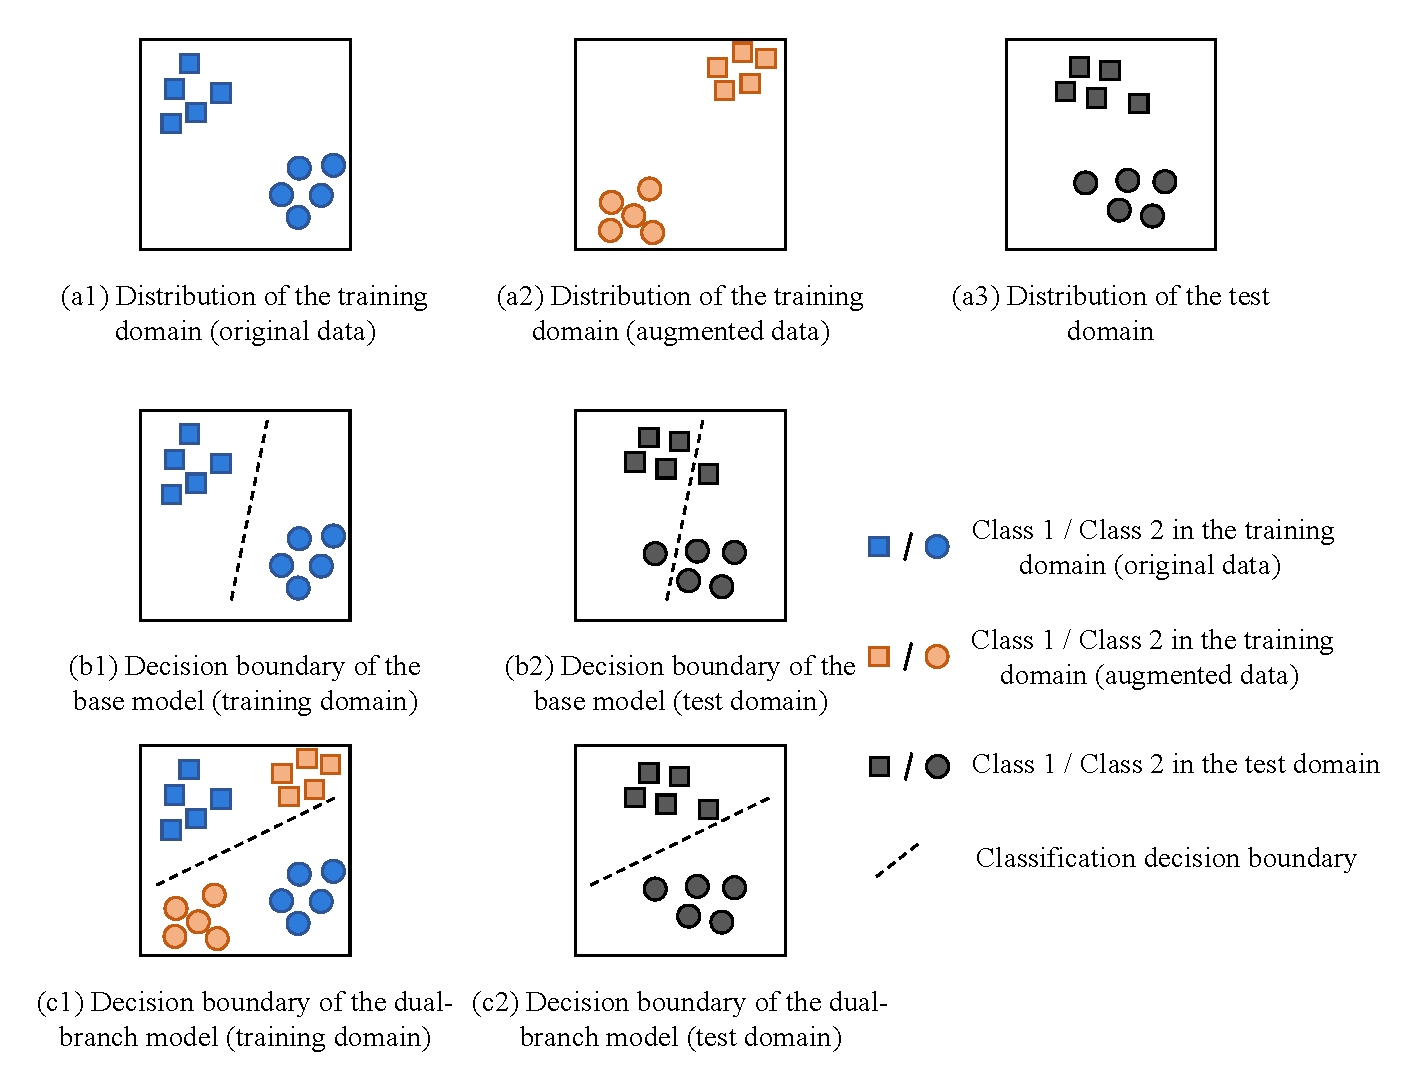
\includegraphics[width=0.72\textwidth]{images/media/image1_padded.pdf}
\caption{Schematic illustration of the decision boundaries of a conventional model and a dual-branch model under domain shift. (a) shows the distribution relationship among original source-domain images (training set), augmented source-domain images, and the target domain (test set), where augmented source-domain images are used to simulate possible distribution shifts in the target domain. (b) When the model is trained only with original source-domain images, the learned decision boundary may not fit the target domain and can therefore cause classification errors on target-domain samples. (c) By constructing a dual-branch structure with original and augmented source-domain images and incorporating contrastive learning with CAM guidance, \protect\revision{the model aims to learn transferable disease-related features and a decision boundary that is more applicable to unseen domains.}}
\label{fig:intro-domain-gap}
\end{figure}

3. \revision{Indeed, the need to protect sensitive patient information in cross-institutional use of medical data is a key reason for these restrictions on data sharing and collaborative training across multiple sources} \cite{_Ref213949393}. \revision{Medical images contain information about patients' health and clinical care, placing stringent privacy requirements on their access and use. In cross-domain learning, adaptation methods that require target-domain samples introduce additional data access and interaction requirements, which may increase privacy risks and complicate the integration of privacy mechanisms, while the privacy constraints introduced in this process may further affect model optimization and recognition performance. Another key challenge is therefore to reduce data exposure during cross-domain learning and deployment while protecting training information and preserving cross-domain recognition performance as much as possible.}

\revision{To address these interrelated requirements, this study presents a privacy-preserving interpretable single-domain generalization framework for multi-label ocular disease recognition. The framework adopts a single-source learning route that combines multi-label representation learning with protection of source-domain training information. Within this setting, CAM-guided dual-view feature filtering and disease-label representation consistency are jointly optimized to learn disease-discriminative features under appearance variations.}

For the common issue of multi-disease co-occurrence in ocular disease recognition, \revision{the framework incorporates a Transformer-based} Adaptive Label-Feature Relevance Construction (ARC) module. It models label relevance using Transformer self-attention and fuses label semantics with corresponding image features using Transformer cross-attention, thereby constructing disease co-occurrence dependencies at both the label and feature levels to reduce false positives and false negatives in multi-label recognition.

\revision{To learn representations that transfer across imaging conditions,} \revision{the framework includes a Dual-Branch} Guided Domain-Invariant Feature Extraction (DFE) module. This module is trained using only a single source domain and constructs a dual-branch structure from original source-domain images and style-disturbed augmented source-domain images, as shown in \hyperref[fig:intro-domain-gap]{Fig.~\ref*{fig:intro-domain-gap}.a1} and \hyperref[fig:intro-domain-gap]{Fig.~\ref*{fig:intro-domain-gap}.a2}, to learn their shared representations at the feature level. Meanwhile, Class Activation Mapping (CAM) is introduced as prior guidance to encourage the model to focus on disease-related regions and suppress the learning of domain-specific noise. This enables the model to form a decision boundary that is more suitable for unseen-domain distributions (\hyperref[fig:intro-domain-gap]{Fig.~\ref*{fig:intro-domain-gap}.c1}) and to maintain stable recognition performance on unseen domains (\hyperref[fig:intro-domain-gap]{Fig.~\ref*{fig:intro-domain-gap}.c2}). In addition, CAM visualizes model-attended regions and enhances model interpretability.

\revision{To address privacy requirements in cross-domain applications, the single-source domain generalization approach adopted in this study restricts training updates to source-domain data. This reduces the need to access target-domain training data or pool raw data across institutions, providing protection through data isolation. Research on medical single-source domain generalization likewise identifies privacy and data access constraints as motivations for this setting} \cite{_RefMatsun2025ConDiSR}. \revision{Building on this setting, the framework incorporates an Adaptive Gaussian Differential Privacy (AdaGDP) mechanism into the joint optimization of DFE and ARC. Gradient clipping and dynamic noise injection impose privacy constraints on parameter updates to further protect source-domain training information. The noise schedule and optimization settings aim to minimize the impact of privacy-preserving training on cross-domain recognition performance.}

\revision{Under non-private training, experiments on several representative fundus image datasets show improved recognition performance over the corresponding ResNet50 baselines in the evaluated in-domain and cross-domain settings. CAM visualizations illustrate the regions attended by the model. Privacy-preserving experiments further quantify the recognition performance achieved at the reported privacy budgets.}

The main contributions of this study are summarized as follows:

\begin{enumerate}
\item \revision{We develop an Adaptive Label-Feature Relevance Construction (ARC) module that uses disease-label queries to extract corresponding image representations. A cross-view consistency constraint encourages the representation associated with each disease label to remain close across the original and augmented images, linking feature stability learning to multi-label discrimination.}

\item \revision{We design a Dual-Branch Guided Domain-Invariant Feature Extraction (DFE) module that combines CAM guidance with a mask based on normalized feature differences to filter features from the original and augmented images. It provides ARC with representations that are relatively stable under the selected appearance perturbations and uses CAM to visualize the regions attended by the model.}

\item \revision{We combine single-source generalization with privacy-constrained optimization of the joint DFE and ARC model. Source-only training updates limit the data required for cross-domain learning, while AdaGDP applies gradient clipping and scheduled noise injection to protect source-domain training information. The training design is evaluated in terms of privacy budget and recognition performance.}
\end{enumerate}

The remainder of this paper is organized as follows. Section 2 reviews recent related work. Section 3 presents the proposed method in detail, and Section 4 reports the complete experimental settings and results. Section 5 concludes the paper and discusses future work.
